\documentclass{article}
%
%
%	maxwells_equations.tex
%
%	David Meyer
%	dmm613@gmail.com
%	19 Sep 2023
%
%
%   get various packages
%
\usepackage[margin=1.0in]{geometry}                                     % adjust margins
\geometry{letterpaper}                                                  % or a4paper or a5paper or ... 
\usepackage{url}                                                        % need this to use URLs in bibtex
\usepackage{setspace}                                                   % need this for \setstrech{...}
\usepackage{scrextend}                                                  % need this for addmargin
\usepackage[export]{adjustbox}                                          % need this to get frame for includegraphics
%
%   tikz et al
%
\usepackage{tikz}
\usetikzlibrary{calc,patterns,angles,quotes,shapes,math,decorations,
                through,intersections,lindenmayersystems,backgrounds,
                hobby}
\tikzset{>=latex}                                                       % default to LaTeX arrow head
\usepackage{circuitikz}                                                 % draw circuits    
\usepackage{pgfplots}
%
%	more math stuff
%
\usepackage{amsmath,amsfonts,amssymb,amsthm}
\usepackage{bm}
\usepackage{mathtools}
\usepackage{commath}                                                    % get \norm{x}
\usepackage{fixmath}                                                    % get \mathbold
\usepackage{gensymb}                                                    % get \degree
\usepackage{mathrsfs}
\usepackage{hyperref}
\usepackage{subcaption}
\usepackage{authblk}                                                    % comment out if using beamer (stops \author{} from working in beamer)
\usepackage{graphicx}
\usepackage{hyperref}
\usepackage{alltt}
\usepackage{xcolor}
\usepackage{float}
\usepackage{braket}
\usepackage{siunitx}
\usepackage{relsize}
\usepackage{multirow}
\usepackage{esvect}
\usepackage{enumitem}                                                   % use characters instead of numbers in enumerate
\usepackage{changepage}                                                 % needed for \begin{adjustwidth}{-3.25em}{-2.0em} (left justify)
%
%	Describe floating point parameters, \fpeval
%
\ExplSyntaxOn
\cs_set_eq:NN \fpeval \fp_eval:n
\ExplSyntaxOff
%
%	Get the x and y components out of a coordinate, e.g.
%
%	\coordinate (EP) at (8,5);
%	\gettikzxy{(EP)}{\slopex}{\slopey}
%
\makeatletter
\newcommand{\gettikzxy}[3]{%
  \tikz@scan@one@point\pgfutil@firstofone#1\relax
  \edef#2{\the\pgf@x}%
  \edef#3{\the\pgf@y}%
}
\makeatother
%
%
%	Watermarks
%
% \usepackage{draftwatermark}
% \SetWatermarkText{Draft}
% \SetWatermarkScale{5}
% \SetWatermarkLightness {0.9} 
% \SetWatermarkColor[rgb]{0.7,0,0}
%
%
%	theorems, definitions, etc
%
\theoremstyle{definition}
\newtheorem{theorem}{Theorem}[section]
\newtheorem{definition}{Definition}[section]
\newtheorem{proposition}{Proposition}[section]
\newtheorem{lemma}{Lemma}[section]
\newtheorem{example}{Example}[section]
\newtheorem{remark}{Remark}[section]
%
%	For drawing matrix products 
%
\newcommand*{\vertbar}{\rule[-1ex]{0.5pt}{2.5ex}}
\newcommand*{\horzbar}{\rule[.5ex]{2.5ex}{0.5pt}}

%
%	The following code allows you to do
%
%	\begin{bmatrix}[r] (or [c] or [l])
%
\makeatletter
\renewcommand*\env@matrix[1][c]{\hskip -\arraycolsep
  \let\@ifnextchar\new@ifnextchar
  \array{*\c@MaxMatrixCols #1}}
\makeatother
%
%	make \arg{min,max}_{n \to \infty} work nicely
%
\newcommand{\argmax}{\operatornamewithlimits{argmax}}
\newcommand{\argmin}{\operatornamewithlimits{argmin}}
%
%	handy commands
%
\newcommand*{\Scale}[2][4]{\scalebox{#1}{$#2$}}
\DeclareMathOperator{\E}{\mathbb{E}}
\DeclareMathOperator{\bda}{\Big \downarrow}										% big down arrow
\newcommand{\veq}{\mathrel{\rotatebox{90}{$=$}}}
%
%	Title, author and date
%
\title{A Few Notes on Maxwell's Equations}
\author{David Meyer \\ 
	{\small \vspace{-2.75mm} \href{mailto:dmm613@gmail.com}{dmm613@gmail.com}}}
\date{Last Update: \today \\
	{\small \vspace{1.00mm} Initial Version: September 19, 2022}}
%
% \date{Last update: \today}
%
%
%
\begin{document}
\maketitle
%
%	Global constants
%
\def \vE{\mathbf{E}}
\def \vB{\mathbf{B}}
\def \vJ{\mathbf{J}}
\def \vi{\mathbf{\hat{i}}}
\def \vj{\mathbf{\hat{j}}}
\def \vk{\mathbf{\hat{k}}}
%
%
%
\section{Introduction}
\label{sec:introduction}
Maxwell's equations are a set of four fundamental equations that
describe the behavior of electric and magnetic fields in
classical electromagnetism. They were formulated by the Scottish
physicist James Clerk Maxwell in the 19th century and are crucial
in understanding the behavior of electromagnetic waves, such as
light (an idea previously articulated by Faraday
\cite{faraday_and_the_em_theory_of_light}). Maxwell's equations
are typically written in both differential and integral forms
\cite{wikipedia:maxwells_equations}.

\bigskip
\noindent
Maxwell's equations are fundamental to classical electromagnetism
and have played a crucial role in the development of modern
physics and technology, including the understanding of
electromagnetic waves, the design of electrical circuits, and the
development of technologies such as radio, television, and
wireless communication, to name a few.

\bigskip
\noindent
The rest of this note is organized as follows: Section
\ref{sec:definitions} provides a few definitions needed to
discuss Maxwell's equations. Section
\ref{sec:maxwells_equations_differential_form} discusses the
differential form of Maxwell's equations, and Section
\ref{sec:maxwells_equations_integral_form} discusses the integral
form of Maxwell's equations. Section \ref{sec:emwaves} discusses
a few of the properties of electromagnetic waves. Section 
\ref{sec:heaviside_contribution} briefly discusses Oliver
Heaviside's contributions to Maxwell's equations. Finally,
Section \ref{sec:conclusions} outlines some conclusions and final
thoughts.
%
%
%
\section{Definitions}
\label{sec:definitions}


\begin{definition}A \emph{field} is an algebraic
structure\footnote{See Appendix A for a brief review of a few
important algebraic structures.}  consisting of a non-empty set
$\mathbb{K}$ equipped with two binary operations, $+$ (addition)
and $\cdot$ (multiplication), satisfying the
conditions\footnote{See Appendix B for more on groups and
fields.}:

\medskip
\begin{itemize}
\item [] (A) $(\mathbb{K},+)$ is an Abelian group with identity element $0$ 
             (called zero).
\item [] (M) $(\mathbb{K} \backslash \{0\}, \cdot)$ is an Abelian group with 
             identity element 1.
\item [] (D) The distributive law $a(b+c)=ab+ac$ holds for all $a,b,c \in \mathbb{K}$.
\end{itemize}

\medskip
\noindent
Examples of important fields include

\smallskip
\begin{itemize}
\item $\mathbb{Q}$,     the field of rational numbers
\item $\mathbb{R}$,     the field of real numbers
\item $\mathbb{C}$,     the field of complex numbers
\item $\mathbb{Z}_{p}$, the field of integers mod $p$ for prime $p$ 
\end{itemize}
\end{definition}

\bigskip
\noindent
Aside: Interestingly, every field is an integral domain, and
integral domains have cancellation laws. 

\bigskip
\noindent
Ok, but why? Well, consider Lemma \ref{lemma:zero_divisors}:

\smallskip
\begin{lemma}
$R$ has a cancellation law iff $R$ is an integral domain.
\label{lemma:zero_divisors}
\end{lemma}


\noindent
\textbf{Proof.} Consider the $\Rightarrow$ and $\Leftarrow$ cases:

\begin{itemize}
\item [($\Rightarrow$)] Suppose $R$ has a cancellation law 
with $a,b \in R$, $a \neq 0$ and assume that $ab = 0$. Then

\vspace{-0.25cm}															% why is there too much vertical space here?
\begin{equation*}
\begin{array}{rcll} 
ab
&=& 0 								
			&\hspace{2em} \mathrel{\#} \text{by assumption} \\
[5pt]
&\Rightarrow& a \cdot b = a \cdot 0 
			&\hspace{2em} \mathrel{\#} 0 = a \cdot 0 \\
[5pt]
&\Rightarrow& b = 0 				
			&\hspace{2em} \mathrel{\#} \text{(cancel 
			$a \Rightarrow a$ is not a zero divisor) 
			$\Rightarrow R$ is an integral domain} \\
\end{array}
\end{equation*}

\medskip
\noindent
Thus $R$ has a cancellation law $\Rightarrow$ $R$ is an integral 
domain.

\medskip
\noindent
\item [($\Leftarrow$)] Suppose $R$ is an integral domain with $a,b,c \in R$, 
$a \neq 0$ and assume that $ab = ac$. Then 

\begin{equation*}
\begin{array}{rcll} 
ab
&=& ac                                                  
			&\hspace{2em} \mathrel{\#} \text{by assumption} \\
[5pt]
&\Rightarrow& ab-ac = 0
			&\hspace{2em} \mathrel{\#} \text{subtract $ac$ from both sides} \\
[5pt]
&\Rightarrow& a\cdot(b-c) = 0
			&\hspace{2em} \mathrel{\#} \text{factor out $a$} \\
[5pt]
&\Rightarrow& b-c = 0
			&\hspace{2em} \mathrel{\#} \text{$R$ has no zero divisors and 
				$a \neq 0 \Rightarrow b-c$ must equal zero} \\
[5pt]
&\Rightarrow& b = c 
			&\hspace{2em} \mathrel{\#} \text{$(ab=ac \Rightarrow b = c)
			\Rightarrow R$ has a cancellation law}
\end{array}
\end{equation*}

\medskip
\noindent
Thus $R$ is an integral domain $\Rightarrow$ $R$ has a cancellation 
law. $\blacksquare$
\end{itemize}

\bigskip
\begin{definition}
A vector space $V$ over a field $\mathbb{K}$ is an algebraic
structure consisting of a non-empty \\ set $V$ equipped with a
binary operation $+$ (vector addition) and a scalar
multiplication operation \\ $(a,v) \in \mathbb{K} \times V
\mapsto av \in V$ such that the following rules hold:


\bigskip
\noindent
(VA) $(V,+)$ is an Abelian group with identity element
$\mathbf{0}$ (the zero vector).  

\bigskip
\noindent
(VM) Rules for scalar multiplication:

\medskip
\begin{itemize}
\item [] (VM0) Closure: For any $a   \in \mathbb{K}$ and $v \in V$ there is a unique element $av \in V$.
\item [] (VM1) $\text{Distributivity}_{1}$: For any $a \in \mathbb{K}$ and $u,v \in V$ we have $a(u+v)=au+av$.
\item [] (VM2) $\text{Distributivity}_{2}$: For any $a,b \in \mathbb{K}$ and $v \in V$ we have $(a+b)v=av+bv$.
\item [] (VM3) Associativity: For any $a,b \in \mathbb{K}$ and $v \in V$ we have $(ab)v=a(bv)$.
\item [] (VM4) Identity: For any $v \in V$ we have $1v = v$ (where $1$ is the identity element of $\mathbb{K}$).
\end{itemize}
\end{definition}

\medskip
\noindent
Since vector spaces have two kinds of elements, namely elements
of $\mathbb{K}$ and elements of $V$, we distinguish them by
calling the elements of $\mathbb{K}$ scalars and the elements of
$V$ vectors.

\bigskip
\noindent
A vector space over the field $\mathbb{R}$ is often called a real
vector space while a vector space over $\mathbb{C}$ is called a
complex vector space.

\subsection{Vectors}
In this section we'll define the vector notation that we will use
in these notes as well as a few important vector operations.

\smallskip
\subsubsection{Notation} 

\medskip
\noindent
In these notes we will use boldface to represent a vector.
Specifically, we will use $\mathbf{a} = (a_1,a_2,\hdots, a_n)$ to
represent a column or row vector in some $n$-dimensional space
(usually $\mathbb{R}$ or $\mathbb{C}$). If $\mathbf{a}$ is a
column vector then in matrix format

\begin{flalign*}
\mathbf{a} = 
\underbrace {
\begin{bmatrix} 
a_1 \\
a_2 \\
\vdots \\
a_n
\end{bmatrix}}_{n \times 1}
\end{flalign*}


\medskip
\noindent
If $\mathbf{a}$ is a row vector then in matrix format

\begin{flalign*}
\mathbf{a} = 
\underbrace{
\begin{bmatrix} 
a_1 \; a_2 \; \hdots \; a_n
\end{bmatrix}}_{1 \times n}
\end{flalign*}

\bigskip
\noindent
The \emph{transpose} of a vector $\mathbf{a}$,
$\mathbf{a}^{\intercal}$, is defined as follows: 
If $\mathbf{a}$ is a column vector then

\begin{flalign*}
\mathbf{a}^{\intercal} = 
\begin{bmatrix} 
a_1 \; a_2 \; \hdots \; a_n
\end{bmatrix}
\end{flalign*}

\smallskip
\noindent
Alternatively, if $\mathbf{a}$ is a row vector then

\begin{flalign*}
\mathbf{a}^{\intercal} = 
\begin{bmatrix} 
a_1 \\
a_2 \\
\vdots \\
a_n
\end{bmatrix}
\end{flalign*}


\bigskip
\noindent
Adding a "hat" to a vector denotes the unit vector. That is, for
a vector $\mathbf{u}$, $\hat{\mathbf{u}}$ is defined to be

\medskip
\begin{equation}
\hat{\mathbf{u}} := \dfrac{\mathbf{u}}{\| \mathbf{u} \|}
\label{eqn:hat}
\end{equation}

\bigskip
\noindent
where $\norm{\mathbf{u}}$ is the Euclidean Norm
of the vector $\mathbf{u}$ (Definition
\ref{def:euclidean_norm}). In words: $\hat{\mathbf{u}}$ 
is a vector of unit length in the $\mathbf{u}$ direction. 



\bigskip
\begin{definition}
\label{def:euclidean_norm}
{\bf Euclidean Norm:} $\|\mathbf{x}\|$


\bigskip
\noindent
The Euclidean norm of a vector $\mathbf{x} = (x_1,x_2,\ldots,
x_n) \in \mathbb{R}^{n}$ is defined to be

\bigskip
\begin{equation*}
\|\mathbf{x}\| := \sqrt{\mathbf{x} \cdot \mathbf{x}} =
\sqrt{\sum\limits_{j = 1}^{n} x_{j}^{2}}
\label{eqn:magnitude}
\end{equation*}
\end{definition}


\subsubsection{Canonical Unit/Basis Vectors}
$\vi$, $\vj$, and $\vk$ 
are defined to be the unit vectors in $\mathbb{R}^3$ in the $x$,
$y$, and $z$ directions respectively. Note that $\vi$, 
$\vj$, and $\vk$ are also the canonical 
basis vectors for $\mathbb{R}^3$ and have column vector format 
\cite{notes:basis}:

\bigskip
\begin{equation*}
{\displaystyle \mathbf {\hat {i}} 
= {\begin{bmatrix}1\\0\\0\end{bmatrix}},\,\,
\mathbf {\hat {j}} = {\begin{bmatrix}0\\1\\0\end{bmatrix}},\,\,
\mathbf {\hat {k}} = {\begin{bmatrix}0\\0\\1\end{bmatrix}}}
\end{equation*}

\medskip
\bigskip
\noindent
I have also seen $\mathbf{e}_i$ used to represent the $i^{th}$
basis vector in $\mathbb{R}^n$. So $\mathbf{e}_i$ is a vector
with a one in the $i^{th}$ position and a zero in each of the
other $n - 1$ positions.  In $\mathbb{R}^3$ this means that
$\mathbf{e}_1 = \vi$, $\mathbf{e}_2 =
\vj$, and $\mathbf{e}_3 = \vk$.


\bigskip
\noindent
In general, the standard basis (which is sometimes called the
computational basis) for the $n$-dimensional Euclidean space
consists of the ordered set of $n$ distinct vectors

\medskip
\begin{equation*}
\{\mathbf {e} _{i}: 1 \leq i \leq n\}
\end{equation*}

\bigskip
\noindent
where $\mathbf{e}_i$ is the $i^\text{th}$ basis vector, that is,
it has a one in the $i^\text{th}$ coordinate (position) and zeros
everywhere else\footnote{This is called a "one-hot" encoding in
machine learning, where the $i$'s might be the classes in a
classification problem.}. The $\mathbf{e}_i$ have column vector
format


\begin{flalign*}
\mathbf{e}_{1} = 
\begin{bmatrix} 
1 \\
0 \\
\vdots \\
0 \\
0
\end{bmatrix} \!\! , \;
\mathbf{e}_{2} = 
\begin{bmatrix} 
0 \\
1 \\
\vdots \\
0 \\
0
\end{bmatrix} \!\! , 
\hdots  , \; 
\mathbf{e}_{n-1} =
\begin{bmatrix} 
0 \\
0 \\
\vdots \\
1 \\
0
\end{bmatrix} \!\! , \;
\mathbf{e}_{n} =
\begin{bmatrix} 
0 \\
0 \\
\vdots \\
0 \\
1
\end{bmatrix}
\end{flalign*}


\bigskip
\noindent
Using these definitions we can define the parametric form of some
curve $C$ in $\mathbb{R}^3$, $\mathbf{r}(t)$, as follows:

\medskip
\begin{equation*}
\mathbf{r}(t) = g(t) \, \vi + h(t) \, \vj + k(t) \, \vk.
\end{equation*}

\bigskip
\noindent
where $t \in [a,b]$ and $g(t)$, $h(t)$, and $k(t)$ are scalar
functions\footnote{A scalar function is a function $f$ such that
$f: \mathbb{R}^n \to \mathbb{R}$.}.


\bigskip
\noindent
Another common notation for vectors is $\vec{r}(t)$, where
$\vec{r}(t)$ might be defined as follows:


\bigskip
\begin{equation*}
\vec{r}(t) = g(t) \, \vi +h(t) \, \vj + k(t) \, \vk 
\end{equation*}

\subsection{A Few Definitions}
\label{subsec:a_few_definitions}

\begin{table} [H]
  \centering                                                                                    % center the figure
  \renewcommand{\arraystretch}{2.5}                                                             % get some space in the table cells
  \resizebox{0.80 \textwidth}{!} {                                                              % resize figure if you want
     \begin{tabular} {| c | c  | c | c |}
      \hline
      {\Large \bf Symbol} & {\Large \bf What} & {\Large \bf Dimensions} & {\Large \bf Notes} \\
      \hline \hline
      $\vB$        & Magnetic field             & Newton/m/Ampere       & $\text{N} = \text{kg} \cdot \text{m}
                                                                                \cdot \text{s}^{-2}$ \\ 
      \hline
      $\vE$        & Electric field             & Newton/Coulomb        & $\text{C} = \text{A} \cdot \text{s}$ \\ 
      \hline
      $\vJ$        & Current density            & Ampere/$\text{m}^2$   & $\text{A} = 6.241509074 \times 10^{18} \; 
      																			\text{\bf e}/\text{s}$ \\
      \hline
      $\rho$       & Charge density             & Coulomb/$\text{m}^3$  & $\text{C} = 6.241509074 \times 10^{18} \; 
      																			\text{\bf e}$ \\ 
      \hline
      $c$          & Speed of light in a vacuum & m/s                   & $c = 2.99792458 \times 10^{8} \; \text{m/s}$ \\
      \hline
      $\epsilon_0$ & Permittivity of free space & Farad/m               & $\epsilon_0 = 8.8541878128 \times 10^{-12} \; \text{F/m}$ \\
      \hline
      $\mu_0$      & Permeability of free space & Henry/m               & $\mu_0 = 4\pi \times 10^{-7} \; \text{H/m}$ \\
      \hline
    \end{tabular}
   }                                                                    % end resizebox
  \caption{A Few Definitions}
  \label{tab:definitions}
\end{table}

\bigskip
\subsubsection{Electric and Magnetic Constants in Maxwell's Equations}
\label{subsubsec:electric_and_magnetic_constants}
Maxwell's equations are usually defined using three constants:
the speed of light ($c$), the electric permittivity of free space
($\epsilon_0$), and the magnetic permeability of free space
($\mu_0$). See Table \ref{tab:definitions}.

\bigskip
\noindent
To calculate the value of these constants, first note that the
magnetic permeability of free space $\mu_0$ is taken to have the
exact value $\mu_0 = 4\pi \times 10^{-7} \; \text{H}/\text{m}$
(see Table \ref{tab:definitions}).  So $\mu_0$ is
given\footnote{$1 \; \text{Henry/m} = 1 \;
\text{Newton}/\text{Ampere}^2 \text{ so } \mu_0 = 4\pi \times
10^{-7} \; \text{H}/\text{m} \approx 1.25663706143 \times 10^{-6}
\; \text{N}/\text{A}^2$.}. We also know that the speed of light
$c$ is equal to $2.99792458 \times 10^{8} \; \text{m/s}$ so we
also can consider $c$ as given.

\bigskip
\noindent
Next, notice $\epsilon_0$ and $\mu_0$ are not independent but
rather are related to the speed of light by the following
equation \cite{wikipedia:maxwells_equations}:

\medskip
\begin{equation}
c = \dfrac{1}{\sqrt{\mu_0\epsilon_0}}
\label{eqn:c}
\end{equation}

\bigskip
\noindent
Since we know the values of $\mu_0$ and $c$, we can find the
value of $\epsilon_0$ by solving for it in Equation
(\ref{eqn:c}):

\bigskip
\begin{equation}
\epsilon_0 = \dfrac{1}{\mu_0 c^2}
\label{eqn:epsilon_0}
\end{equation}

\bigskip
\noindent
Substituting the values of $\mu_0$ and $c$ into Equation
(\ref{eqn:epsilon_0}) we get that $\epsilon_0 = 8.8541878128
\times 10^{-12} \; \text{F/m}$. 

\bigskip
\noindent
Finally, note that in the presence of polarizable or magnetic
media \cite{wikipedia:polarization}, the effective constants will
have different values. In the case of a polarizable medium,
called a dielectric, the comparison is stated as a relative
permittivity or a dielectric constant. In the case of magnetic
media, the relative permeability may also be stated.


\subsection{Divergence and Curl}
\label{subsec:divergence_and_curl}
For some vector field $\mathbf{F}$, we call $\nabla \cdot
\mathbf{F}$ the divergence of $\mathbf{F}$, while $\nabla \times
\mathbf{F}$ is called the curl of $\mathbf{F}$
\cite{dmm:vector_calculus}. 

\bigskip
\noindent
It is worth noting that the standard
dot (or inner) product is defined as follows:


\medskip
\begin{definition}
{\bf Standard Inner Product:} $\mathbf{a} \cdot \mathbf{b}$

\bigskip
\noindent
The inner product (aka dot product 
or scalar product) of two $n$-dimensional vectors 
$\mathbf{a} = (a_1,a_2,\hdots, a_n)$ and 
$\mathbf{b} = (b_1,b_2,\hdots, b_n)$, usually 
denoted by either $\langle \mathbf{a}, \mathbf{b} 
\rangle$ or $\mathbf{a} \cdot \mathbf{b}$,
is defined to be the scalar value

\medskip
\begin{equation*}
\mathbf{a} \cdot \mathbf{b} := 
	\sum\limits_{j = 1}^{n} a_j b_j
\label{eqn:inner}
\end{equation*}
\end{definition}

\smallskip
\noindent
Since $a_j$ and $b_j$ are scalars (and scalar multiplication
commutes) the inner product commutes:

\bigskip
\begin{equation}
  \mathbf{a} \cdot \mathbf{b}
  = \sum\limits_{j = 1}^{n} a_j b_j
  = \sum\limits_{j = 1}^{n} b_j a_j
  = \mathbf{b} \cdot \mathbf{a} 
\label{eqn:dot_reverse}
\end{equation}


\bigskip
\noindent
This is all good, but here we are using the dot notation for the
divergence and the divergence is missing a key property that the
standard dot product has, namely, commutivity (Equation
(\ref{eqn:dot_reverse})). Specifically, the standard dot product
commutes but the divergence does not:

\medskip
\begin{equation}
\nabla \cdot \mathbf{F} \neq \mathbf{F} \cdot \nabla
\label{eqn:dot_does_not_commute}
\end{equation}

\bigskip
\noindent
One way to see this is to notice that the LHS of Equation
(\ref{eqn:dot_does_not_commute}) is a scalar function while the
RHS is a differential operator.


\bigskip
\section{Maxwell's Equations (differential form)}
\label{sec:maxwells_equations_differential_form}
The differential form of Maxwell's equations assumes the absence
of magnetic or polarizable media since these media can change the
values of the permittivity and the permeability (see Section
(\ref{subsubsec:electric_and_magnetic_constants})). The differential
form of Maxwell's equations is:

\bigskip
\begin{enumerate}
\item {\bf Gauss's Law for Electricity}
\label{item:gauss_law_electricity}

\begin{equation*}
\nabla \cdot \vE = \dfrac{\rho}{\epsilon_0} 	
\end{equation*}

\bigskip
\noindent
In words: a stationary charge ($\rho$) creates an electric 
field ($\vE$) \cite{gauss_law_for_electricity}.


\bigskip
\item {\bf Gauss's Law for Magnetism}
\label{item:gauss_law_magnetism}

\begin{equation*}
\nabla \cdot \vB = 0							
\end{equation*}

\bigskip
\noindent
In words: magnetic monopoles can not 
exist \cite{gauss_law_for_magnetic_fields}.


\bigskip
\item {\bf Faraday's Law of Electromagnetic Induction} 
\label{item:faradays_law_of_induction}

\begin{equation*}
\nabla \times \vE = -\dfrac{\partial \vB}{\partial t}
\end{equation*}

\bigskip
\noindent
In words: a time-varying magnetic field ($\vB$) creates 
an electric field ($\vE$) \cite{faradays_law}.


\bigskip
\item  {\bf Ampere's Law with Maxwell's addition}
\label{item:ampers_law}

\begin{equation*}
\nabla \times \vB = \mu_0 \vJ + \mu_0 \epsilon_0 
\dfrac{\partial \vE}{\partial t}					
\end{equation*}

\bigskip
{\setstretch{1.60}
\noindent
In words: an electric current ($\vJ$) or a time-varying 
electric field ($\vE$) creates a magnetic field ($\vB$) \cite{amperes_law}. 
Maxwell's addition to Ampere's law is the term $\mu_0 \epsilon_0 \dfrac{\partial 
\vE} {\partial t}$ (time-varying electric fields produce magnetic
fields).	
\par}
\end{enumerate}

\smallskip
\section{Maxwell's Equations (integral form)}
\label{sec:maxwells_equations_integral_form}

\begin{enumerate}
\item {\bf Gauss's Law for Electricity}

\begin{equation*}
\oint_{C} \vE \;  d\mathbf{A}= \dfrac{Q_{\text{enclosed}}}{\epsilon_0}
\end{equation*}

\medskip
\noindent
where $Q_{\text{enclosed}}$ is the enclosed charge. This equation
implies that the electric field lines do not form a continuous
closed path. In words: isolated positive or negative charges can 
exist.


\bigskip
\item {\bf Gauss's Law for Magnetism}

\begin{equation*}
\oint_{C} \vB \;  d\mathbf{A} = 0
\end{equation*}

\medskip
\noindent
This equation says that magnetic lines of force form a
continuous closed path. In words: no isolated magnetic 
monopole can exist.


\bigskip
\item {\bf Faraday's Law of Electromagnetic Induction}

\begin{equation*}
\oint_{C} \vE \; d\mathbf{l} = -\dfrac{d}{dt} \Phi_{\vB}
\end{equation*}

\medskip
\noindent
where $\Phi_{\vB}$ is the magnetic flux through a closed path.
This equation says that the line integral of the electric field
around any closed path is equal to the rate of change of magnetic
flux through the closed path bounded by the surface.

\bigskip
\item {\bf Ampere's Law with Maxwell's addition}

\begin{equation*}
\oint_{C} \vB \; d\mathbf{l} = \mu_0 I_{\text{enclosed}} + 
\mu_0\epsilon_0 \dfrac{d}{dt} \int_{S} \vE \;  d\mathbf{A}
\end{equation*}


\medskip
\noindent
where $I_{\text{enclosed}}$ is the enclosed current.  This
equation says that both conduction and displacement
current can produce a magnetic field.
\end{enumerate}

\smallskip
\section{Electromagnetic Waves}
\label{sec:emwaves}
Classical electromagnetic waves, often referred to simply as
electromagnetic waves, are a fundamental concept in classical
physics that describes the behavior of electromagnetic radiation,
including light, without considering the quantum mechanical
nature of light (as described by quantum electrodynamics). These
waves are described by classical electromagnetism, primarily
through the equations developed by Maxwell in the $19^{\text{th}}$ 
century \cite{wikipedia:maxwells_equations}.

\bigskip
\noindent
The key characteristics and features of classical electromagnetic 
waves include: 

\begin{itemize}
\item {\bf Wave Equation}: The behavior of classical
electromagnetic waves is described by Maxwell's equations, which
consist of four fundamental equations (see Sections 
\ref{sec:maxwells_equations_differential_form} and 
\ref{sec:maxwells_equations_integral_form}):

\begin{enumerate}
\item Gauss's Law for Electricity 
\item Gauss's Law for Magnetism
\item Faraday's Law of Electromagnetic Induction
\item Ampère's Law with Maxwell's addition
\end{enumerate}

\item {\bf Wave Propagation}: Classical electromagnetic waves are
solutions to Maxwell's equations and can propagate through space
as self-sustaining waves of electric and magnetic fields. These
waves travel at the speed of light in a vacuum, $c$, which is
approximately $3.0 \times 10^8 \; \text{m/s}$.

\item {\bf Transverse Waves}: Electromagnetic waves are
transverse waves, which means that the oscillations of the
electric and magnetic fields are perpendicular to the direction
of wave propagation. This is depicted in Figure
\ref{fig:electromagnetic_wave_propagation}. Contrast with
longitudinal waves, where the oscillations are along the 
direction of propagation.

\item {\bf Continuous Spectrum}: Classical electromagnetic waves
encompass a continuous spectrum of frequencies and wavelengths,
from extremely low-frequency radio waves to extremely
high-frequency gamma rays. Each portion of the spectrum
corresponds to different types of electromagnetic radiation.

\item {\bf Wave Polarization}: Electromagnetic waves can be
polarized, meaning that the electric field oscillates in a
specific plane as the wave propagates. Polarization can be
linear, circular, or elliptical, depending on the orientation of
the electric field vector.

\item {\bf Superposition}: Like other waves, classical
electromagnetic waves obey the principle of superposition, which
means that multiple waves can combine to form a new wave through
constructive or destructive interference \cite{dmm:bloch_sphere}.

\item {\bf Energy Transport}: Electromagnetic waves carry energy
as they propagate through space. The intensity of the wave, which
represents the energy per unit area per unit time, is related to
the amplitude of the electric and magnetic fields.

\item {\bf Wave Reflection, Refraction, and Diffraction}:
Classical electromagnetic waves exhibit behaviors such as
reflection when they encounter boundaries, refraction when
passing from one medium to another, and diffraction when
encountering obstacles. These phenomena can be described by
classical wave optics.
\end{itemize}
%
%	draw an electromagnetic wave
%
\bigskip
\begin{figure}[H]                                                               % wrap the wave in a figure
    \centering                                                                  % center the figure
    \fbox{                                                                      % put a box around the figure
        \resizebox{0.75 \textwidth}{!} {                                        % resize figure if you want
%
%	Draw the picture
%
                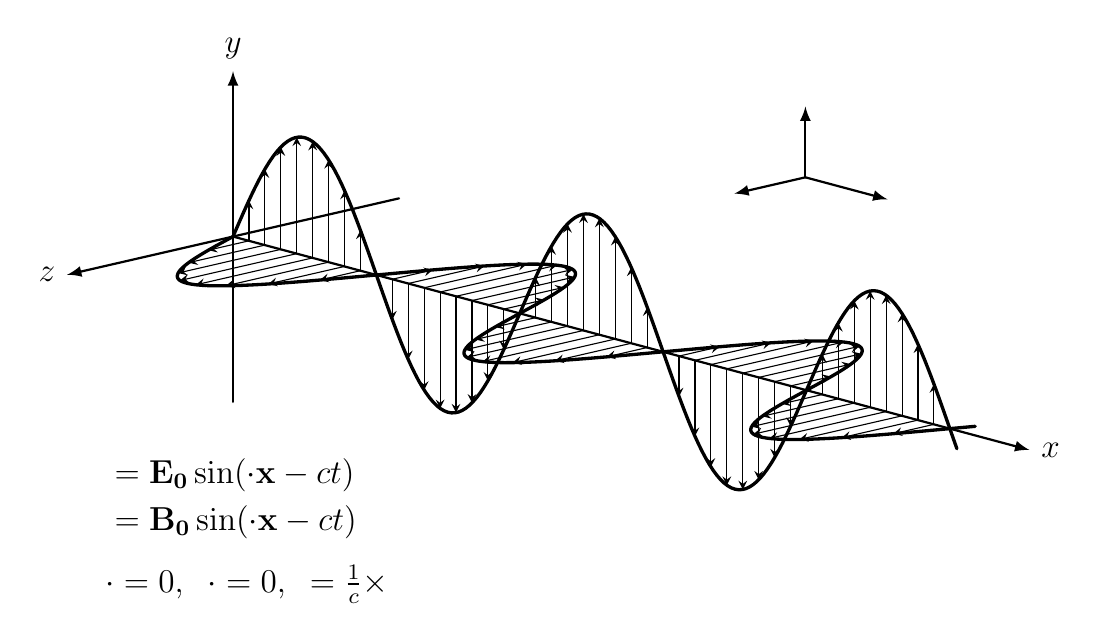
\begin{tikzpicture}[x=(-15:1.2), y=(90:1.0), z=(-150:1.0),      % set a few TikZ parameters
                                        line cap=round, line join=round,
                                        axis/.style={black, thick,->},
                                        vector/.style={>=stealth,->}]
%
%	Definitions
%
%
%	Coordinates
%
                        \coordinate (O) at (0,0,0);                             % origin
%
%	Constants
%
  			\large
  			\def \A{1.5}
                        \def \nNodes{5}
  			\def \nVectorsPerNode{8}
  			\def \N{\nNodes*40}
  			\def \xmax{\nNodes*pi/2*1.01}
  			\pgfmathsetmacro\nVectors{(\nVectorsPerNode+1)*\nNodes}
 %
 %	Draw the main axes
 %
  			\draw[axis] (O)           -- ++(\xmax*1.1,0,0) node[right] {$x$};
  			\draw[axis] (0,-\A*1.4,0) -- (0,\A*1.4,0)      node[above] {$y$};
  			\draw[axis] (0,0,-\A*1.4) -- (0,0,\A*1.4)      node[left]  {$z$};
 %
 %	Draw the small axes
 %
 			\def\xOffset{{(\nNodes-2)*pi/2}}
			\def\yOffset{\A*1.2}
			\def\zOffset{\A*1.2}
			\draw[axis] (\xOffset,\yOffset,-\zOffset) -- ++(\A*0.6,0,0) node[right] {$\vi$};
			\draw[axis] (\xOffset,\yOffset,-\zOffset) -- ++(0,\A*0.6,0) node[above] {$\vE$};
			\draw[axis] (\xOffset,\yOffset,-\zOffset) -- ++(0,0,\A*0.6) node[left]  {$\vB$};
 %
 %	Draw the equations
 %
			\node[above right] at (\xOffset,-0.5*\yOffset,4*\zOffset)
				{$\begin{aligned}
					\vE &= \mathbf{E_0}\sin(\vi\cdot\mathbf{x}-ct)\\
					\vB &= \mathbf{B_0}\sin(\vi\cdot\mathbf{x}-ct)\\
				\end{aligned}$};
			\node[below right] at (\xOffset,-0.5*\yOffset,4*\zOffset)
				{$\vE\cdot\vi = 0,\;\; \vB\cdot\vi = 0,\;\; 
					\vB = \frac{1}{c}\vi\times\vE$};
 %
 %	Now draw the waves
 %
			\draw[very thick,variable=\t,domain=0:\nNodes*pi/2*1.01,samples=\N]
    			plot (\t,{\A*sin(\t*360/pi)},0);
			\draw[very thick,variable=\t,domain=0:\nNodes*pi/2*1.01,samples=\N]
    			plot (\t,0,{\A*sin(\t*360/pi)});
%
%	Draw the vectors
%
			\foreach \k [evaluate={\t=\k*pi/2/(\nVectorsPerNode+1);
                         \angle=\k*90/(\nVectorsPerNode+1);
                         \c=(mod(\angle,90)!=0);}]
					in {1,...,\nVectors}{
						\if\c1
							\draw[vector] (\t,0,0) -- ++(0,{\A*sin(2*\angle)},0);
							\draw[vector] (\t,0,0) -- ++(0,0,{\A*sin(2*\angle)});
						\fi
					}
		\end{tikzpicture}
       }                                                                                % end resizebox
    }                                                                                   % end fbox
\caption{Propagation of an electromagnetic wave in the $\vi$ direction}
\label{fig:electromagnetic_wave_propagation}
\end{figure}
%
%
%
\bigskip
\noindent
It's important to note that while classical electromagnetic wave
theory provides an accurate description of many electromagnetic
phenomena, it does not account for the quantum nature of light,
which is described by quantum electrodynamics (QED)
\cite{wikipedia:quantum_electrodynamics}. In certain situations,
particularly at very small scales or in the presence of intense
electromagnetic fields, the quantum nature of light becomes
significant, and classical wave theory may not fully explain the
observed behavior.
%
%
%
\section{Oliver Heaviside's Contributions to Maxwell's Equations}
\label{sec:heaviside_contribution}
Oliver Heaviside made significant contributions to the
understanding and reformulation of Maxwell's equations. His work
helped simplify and clarify these equations, making them more
accessible and useful for engineers and physicists. 

\bigskip
\noindent
A few of Heaviside's important contributions to Maxwell's 
equations include \cite{the_long_road_to_maxwells_equations,
wikipedia:history_of_maxwells_equations}:

\medskip
\begin{itemize}
\item {\bf Vector Notation}: Heaviside introduced the modern
vector notation for Maxwell's equations, which greatly simplified
their mathematical expression. This notation represented electric
and magnetic fields as vectors, making it easier to write and
manipulate the equations. Heaviside's notation is still widely
used today \cite{dmm:vector_calculus}.

\item {\bf Telegrapher's Equations}: Heaviside derived what are
now known as the Telegrapher's Equations, which describe the
behavior of electrical signals in transmission lines, such as
telegraph cables. These equations are a simplified form of
Maxwell's equations and are crucial for understanding the
propagation of electromagnetic waves in transmission lines
\cite{wikipedia:telegraphers_equations}.

\item {\bf Concept of Impedance}: Heaviside introduced the
concept of electrical impedance, which is a measure of how much a
medium resists the flow of alternating current. He showed how
impedance relates to the propagation of electrical signals in
transmission lines and how it affects the reflection and
transmission of signals \cite{impedance}.

\item {\bf Elimination of Quaternions}: Heaviside eliminated the
use of quaternions, a complex mathematical system that Maxwell
had initially used to describe electromagnetic phenomena. He
replaced quaternions with the more intuitive vector notation,
making Maxwell's equations more accessible to a wider audience
\cite{quaternion}.

\item {\bf Improved Understanding of Displacement Current}:
Heaviside clarified the concept of displacement current, which is
a term introduced by Maxwell to account for changing electric
fields. Heaviside's work helped physicists better understand this
concept and its role in the equations
\cite{wikipedia:displacement_current}.

\item {\bf Operational Calculus}: Heaviside is also known for his
significant contributions to the field of electrical engineering
and the development of operational calculus. Operational calculus
is a mathematical technique used to solve differential equations,
especially those that arise in the study of electrical circuits
and systems. The operational calculus is also known as the 
Heaviside calculus in honor of his pioneering work in this area  
\cite{wikipedia:operational_calculus}.

\medskip
\noindent
Operational calculus is primarily concerned with transforming
differential equations into algebraic equations, which are often
easier to manipulate and solve. Heaviside's work helped simplify
the analysis of complex linear systems, making it more accessible
to engineers and scientists.

\medskip
\noindent
Some of the key concepts and techniques associated with
Heaviside's operational calculus include:

\begin{itemize}
\item {\bf Laplace Transforms}: Heaviside introduced the use of
Laplace transforms to solve linear differential equations with
initial conditions. This transformation converts a differential
equation into an algebraic equation, simplifying the solution
process \cite{dmm:dirac_delta_and_laplace_transform}.

\medskip
\item {\bf Differential Operators}: Heaviside introduced the
notion of differential operators, such as the D-operator, 
$D= \frac{d}{dt}$, which allows us to manipulate differential 
equations more efficiently 
\cite{d-operator,wikipedia:differential_operator}.

\medskip
\item {\bf Heaviside Step Function}: Heaviside introduced the
unit step function (also known as the Heaviside step function) 
as a way to represent and model sudden changes in electrical
circuits. The Heaviside step function is shown in Definition 
\ref{def:heaviside_function} and Figures \ref{fig:H(t)}, 
\ref{fig:H(t-a)} and \ref{fig:H(a-t)}.

\bigskip
\begin{definition} {\bf Heaviside Step Function:}
\bigskip
\begin{equation*}
H(t) =
 \begin{cases} 
   0 & t < 0  \\
   1 & t > 0 \\
   \text{undefined or 0.5} & t = 0 \text{ (depending on convention)}
   \end{cases}
\end{equation*}
\label{def:heaviside_function}
\end{definition}

\bigskip
\noindent
The Heaviside step function is shown in Figure \ref{fig:H(t)}.

\bigskip
\begin{figure}[H]
  \centering																			% center the figure
  \resizebox{0.60 \textwidth}{!} {														% resize figure if you want
  \begin{tikzpicture}[scale=2.0]
     \draw [thick,->,dashed] (0,0) -- (0,2);                                            % draw axes
     \draw [thick,->,dashed] (0,0) -- (3,0);                                            % draw axes
     \draw (2,2) node[draw,rectangle] {                                                 % draw function to the right
         $H(t) =  
           \begin{cases} 
               0                       & t < 0  \\
               1                       & t > 0  \\
               \text{undefined or 0.5} & t = 0
           \end{cases}$
       }; 
     \draw (3,0) node [label=right:{$t$}] {};
     \draw (0,2) node [label=above:{$H(t)$}] {};
     \draw [<-,thick,red] (-2,0) -- (0,0);
     \draw [->,thick,red] (0,1) -- (3,1);
     \coordinate (y) at (0,1); \fill [red] (y) circle (1pt);                            % draw a dot on the y axis
     \draw (0,1) node[left] {1};
     \draw [thick,red] (0,0) circle [radius =0.03cm];                                   % draw an open red circle on the x axis
     \draw (0,0) node[below] {$0$};
  \end{tikzpicture}
  }																						% end resizebox
  \caption{The Heaviside Function $H(t)$}
  \label{fig:H(t)}
\end{figure}


\bigskip
\noindent
Frequently we are interested in $H(t-a)$, which is sometimes 
written as $u_{a}(t)$ and is shown in Figure \ref{fig:H(t-a)}.


\bigskip
\begin{figure}[H]
  \centering                                                                            % center the figure
  \resizebox{0.60 \textwidth}{!} {                                                      % resize figure if you want
  \begin{tikzpicture}[scale=2.0]
     \draw [thick,->] (0,0) -- (0,2);                                                   % draw axes
     \draw [thick,<->] (-2,0) -- (3,0);                                                 % draw axes
     \draw (3,2) node[draw,rectangle] {                                                 % draw function to the right
         $H(t-a) =  
           \begin{cases} 
               0                       & t < a  \\
               1                       & t > a \\
               \text{undefined or 0.5} & t = a
           \end{cases}$
       }; 
     \draw (1,0) node[below] {$a$};
     \draw [thick,red] (1,0) circle [radius =0.03cm];                                   % draw an open red circle on the x axis above the "a"
     \draw [dashed] (1,0) -- (1,1);
     \draw (3,0) node [label=right:{$t$}] {};
     \draw (0,2) node [label=above:{$H(t-a)$}] {};
     \draw [thick,red] (-2,0) -- (1,0);
     \draw [->,thick,red] (1,1) -- (3,1);
     \coordinate (xy) at (1,1); \fill [red] (xy) circle (1pt);                          % draw a dot on the y axis
     \draw [dashed] (0,1) -- (2,1);
     \draw [thick,red] (1,1) circle [radius =0.03cm];                                   % draw an open red circle on the x axis
     \coordinate (y) at (0,1); \fill [black] (y) circle (1pt);                          % draw a dot on the y axis
     \draw (0,1) node[left] {1};
  \end{tikzpicture}
  }																						% end resizebox
  \caption{$H(t-a)$}
  \label{fig:H(t-a)}
\end{figure}

\bigskip
\noindent
Another useful version of the Heaviside step function, $H(a - t)$,
is shown in Figure \ref{fig:H(a-t)}.

\bigskip
\begin{figure}[H]
  \centering                                                                            % center the figure
  \resizebox{0.60 \textwidth}{!} {                                                      % resize figure if you want
  \begin{tikzpicture}[scale=2.0]
     \draw [thick,->] (0,0) -- (0,2);                                                   % draw axes
     \draw [thick,<->] (-2,0) -- (3,0);                                                 % draw axes
     \draw (3,2) node[draw,rectangle] {                                                 % draw function to the right
         $H(a - t) =  
           \begin{cases} 
               0 & t > a \\
               1 & t > a \\
               \text{undefined or 0.5} & t = a
           \end{cases}$
       }; 
     \draw (3,0) node [label=right:{$t$}] {};
     \draw (0,2) node [label=above:{$H(a - t)$}] {};
     \draw (1,0) node[below] {$a$};
     \draw [thick,red] (1,0) circle [radius =0.03cm];                                   % draw an open red circle on the x axis above the "a"
     \draw [<-,thick,red] (-2,1) -- (1,1);
     \draw [dashed] (1,0) -- (1,1);
     \draw [->,thick,red] (1,0) -- (3,0);
     \coordinate (xy) at (1,1); \fill [red] (xy) circle (1pt);                          % draw a dot on the y axis 
     \coordinate (y) at (0,1); \fill [black] (y) circle (1pt);                          % draw a dot on the y axis 
     \draw (0,1) node[left,above,xshift=-2.0mm] {1};
     \end{tikzpicture}
  }																						% end resizebox
  \caption{$H(a - t)$}
  \label{fig:H(a-t)}
\end{figure}
\end{itemize}

\bigskip
\noindent
Interestingly, the derivative of the Heaviside function $H(t)$ 
is the Dirac delta function $\delta(t)$. More specifically, 

\begin{equation*}
\dfrac{d}{dt} H(t) = \delta(t)
\end{equation*}

\bigskip
\noindent
Heaviside's work in operational calculus and electrical
engineering significantly influenced the development of modern
control theory and signal processing. His contributions made it
possible to analyze and design electrical and electronic systems
more efficiently.

\bigskip
\noindent
Operational calculus remains an important tool in engineering and
physics, especially in the analysis of linear time-invariant
systems. While the formalism of operational calculus has evolved
since Heaviside's time, his pioneering work laid the foundation
for these developments and continues to be influential in various
engineering disciplines.
\end{itemize}

\bigskip
\noindent
Oliver Heaviside's contributions to Maxwell's equations were
instrumental in simplifying and modernizing the mathematical
description of electromagnetism. His work made it easier for
engineers and scientists to apply these equations to practical
problems and laid the foundation for many developments in
electrical engineering and telecommunications.
%
%
%
\section{Conclusions}
\label{sec:conclusions}
%
%
%
\section{Acknowledgements}
\label{sec:acknowledgements}
Thanks to Larry Lang for suggesting that I add some text about 
Oliver Heaviside's important contributions to Maxwell's equations 
(see Section \ref{sec:heaviside_contribution}). Thanks also
to rrogers (@rrogers@mathstodon.xyz) for pointing out Heaviside's
contributions to the development of operational calculus.
%
%	LaTeX source on overleaf.com
%
\section*{\LaTeX \hspace{0.025 mm} Source}
\url{https://www.overleaf.com/read/fdtbdjmvtryx}
%
%	get a bibliography
%
%	Note:.bib files go in ~/Library/texmf/bibtex/bib with TeXShop (MacTeX).
%	You can also use an absolute path, e.g. \bibliography{/Users/dmm/papers/bib/qc}
%
\bibliographystyle{plain}
\bibliography{qc}
%
%	Appendices 
%
\section*{Appendix A}
\subsection*{A Brief Review of a Few Algebraic Structures}

\begin{center}
\begin{table}[H]
\scalebox{0.85}{
\begin{tabular}{l | c | c | c | c |  c | c}
{{\large \bf Structure}}        & $\textbf{\large ABO}^1$              & {\large \bf Identity}
                                & {\large \bf Inverse}                 & {\large \bf $\text{Distributive}^2$}
                                & {\large\bf $\text{Commutative}^3$}   & {\bf Comments} \\
\hline\hline                                                                                            % separate column names from rows
Semigroup                       & \checkmark & no         & no         & N/A        & no    & $(S,\circ)$ \\
Monoid                          & \checkmark & \checkmark & no         & N/A        & no    & Semigroup plus identity $\in S$ \\
Group                           & \checkmark & \checkmark & \checkmark & N/A        & no    & Monoid plus inverse $\in S$ \\
Abelian Group                   & \checkmark & \checkmark & \checkmark & N/A        & \checkmark $(\circ)$ & Commutative group \\
$\text{Ring}_{+}$               & \checkmark & \checkmark & \checkmark & \checkmark & \checkmark $(+)$     & Abelian group under $+$ \\
$\text{Ring}_{*}$               & \checkmark & yes/no     & no         & \checkmark & no                   & Monoid under $*$ \\
$\text{Field}_{(+,*)}$          & \checkmark & \checkmark $(+,*)$      & \checkmark $(+,*)$ & \checkmark   & \checkmark $(+,*)$
                                             & Abelian group under $+$ and $*$  \\
Vector Space                    & \checkmark & \checkmark $(+,*)$      & \checkmark $(+)$   & \checkmark   & \checkmark $(+)$
                                             & Abelian group under $+$, scalars $\in$ Field \\
Module		                & \checkmark & \checkmark $(+,*)$          & \checkmark $(+)$   & \checkmark   & \checkmark $(+)$
                                             & Abelian group under $+$, scalars $\in$ Ring

\end{tabular}}
\caption{A Few Algebraic Structures and Their Features}
\label{tab:algebraic_structures}
\end{table}
\end{center}

\vspace{-10.0mm}
\noindent
\subsection*{\underline{Abbreviations}}

\medskip
\begin{enumerate}
\item \textbf{ABO:} Associative Binary Operation 
\begin{itemize}
\item $(x \circ y) \circ z = x \circ  (y \circ z)$  
      for all $x, y, z \in S$
\item $x \circ y \in S$ for all $x, y \in S$
      ($S$ is closed under $\circ$)
\end{itemize}

\item \textbf{Distributive:} Distributive Property 
\begin{itemize}
\item Left Distributive Property:  $x * (y+z )= (x*y) + (x*z)$ for
                                   all $x, y, z \in S$
\item Right Distributive Property: $(y + z) * x = (y*x) + (z*x)$
                                   for all $x, y, z \in S$
\item $*$ is \emph{distributive}   over $+$ if $*$ is left and 
                                   right distributive
\end{itemize}

\item \textbf{Commutative:} Commutative Property
\begin{itemize}
\item $x \circ y = y \circ x {\mbox{ for all }}x,y\in S$
\end{itemize}
\end{enumerate}


\noindent
\subsection*{\underline{Notes}}
\begin{itemize}
\item Table \ref{tab:algebraic_structures} implies that $\text{F}
\subset \text{R} \subset \text{G} \subset \text{M} \subset \text{SG}$.
\item Whether or not a ring has a multiplicative identity 
      seems to depend on the field of study. 

\smallskip
\noindent
      In general the definition of a ring $R$ doesn't require a
      multiplicative inverse in $R$ ($a^{-1} \notin R$ for all $a
      \in R$) or that multiplication be commutative in
      $R$. Specifically: $R$ is an Abelian group under $+$ but we
      don't require that multiplication be commutative (while
      $a+b = b+a$ for all $a,b \in R$, we don't require that $ab
      = ba$ for all $a,b \in R$). These are perhaps the main ways
      in which a ring differs from a field. In addition, as
      mentioned above in some cases $R$ need not include a
      multiplicative identity $(1 \notin R)$.

\item $\text{F} \subset \text{VS}$ since the field axioms require
      a multiplicative inverse ($a^{-1}$) while vector spaces do
      not. Fields are also commutative under $*$ and vector
      spaces are not.

\item $\text{VS} \subset \text{Module}$ since the scalars in a
      module come from a ring as opposed to a field like we find
      in vector spaces and $\text{F} \subset \text{R}$
\cite{module_theory_blyth}.
\end{itemize}

\section*{Appendix B}
\subsection*{{\Large Fields and Vector Spaces}}

\smallskip
\subsubsection*{\large \underline {Fields}}
A \emph{field} is an algebraic structure $\mathbb{K}$ in which we can 
add and multiply elements such that the following laws hold:

\bigskip
\noindent
{\bf Addition Laws}
\smallskip
\begin{itemize}
\item [] (FA0) Closure: For any $a,b \in \mathbb{K}$ there is a 
               unique element $a+b \in \mathbb{K}$.
\item [] (FA1) Associativity: For all $a,b,c \in \mathbb{K}$ we have 
               $a+(b+c) = (a+b)+c$.
\item [] (FA2) Identity: There is an element $0 \in \mathbb{K}$ 
               such that $a+0= 0+a = a$ for all  $a \in \mathbb{K}$.
\item [] (FA3) Inverse: For any $a \in \mathbb{K}$ there exists 
               $-a \in \mathbb{K}$ such that $a+(-a) = (-a)+a = 0$.
\item [] (FA4) Commutativity: For any $a,b \in \mathbb{K}$ we have $a+b = b+a$.
\end{itemize}



\medskip
\noindent
{\bf Multiplication laws}
\smallskip
\begin{itemize}
\item [] (FM0) Closure: For any $a, b \in \mathbb{K}$, there is a unique element 
               $ab \in \mathbb{K}$.
\item [] (FM1) Associativity: For all $a,b,c \in \mathbb{K}$ we have $a(bc)=(ab)c$.
\item [] (FM2) Identity: There is an element $1 \in \mathbb{K}$, $1 \ne 0$,
               such that $a1 = 1a = a$ for all $a \in \mathbb{K}$.
\item [] (FM3) Inverse: For any $a \in \mathbb{K}$ with $a \ne 0$, there exists 
               $a^{-1} \in \mathbb{K}$ such that $aa^{-1} = a^{-1}a = 1$.
\item [] (FM4) Commutativity: For any $a,b \in \mathbb{K}$ we have $ab=ba$.
\end{itemize}

\medskip
\noindent
{\bf Distributive law}
\smallskip
\begin{itemize}
\item [] (D) Distributivity: For all $a,b,c \in \mathbb{K}$, we
have $a(b+c) = ab+ac$. 
\end{itemize}

\bigskip
\noindent
Note the similarity of the addition and multiplication laws. We
say that $(\mathbb{K},+)$ is an \emph{Abelian} group if
(FA0)-(FA4) hold.  (FM0)-(FM4) say that $(\mathbb{K} \backslash
\{0\}, \cdot)$ is also an Abelian group (we have to leave out $0$
because as (FM3) says, $0$ does not have a multiplicative
inverse).

\bigskip
\noindent
Examples of fields include $\mathbb{Q}$ (the rational numbers),
$\mathbb{R}$ (the real numbers), $\mathbb{C}$ (the complex
numbers), and $\mathbb{Z}_{p}$ (the integers mod $p$, for $p$ a
prime number).

\bigskip
\noindent
Associated with any field $\mathbb{K}$ is a non-negative integer
called its characteristic, which is defined as follows: the
characteristic of a field $\mathbb{K}$, often denoted
$\text{char} (\mathbb{K})$, is the smallest number of times one
must use the field's (or ring's) multiplicative identity (1) in a
sum to get the additive identity (0). If this sum never reaches
the additive identity the field is said to have characteristic
zero. That is,

\bigskip
\begin{equation*}
\text{char}(\mathbb{K}) = 
    \begin{cases}
        n & \text{$n$ is the smallest positive number such that } 
              \underbrace{1+1+ \cdots + 1}_{n} = 0 \\
        0 & \text{if the sum of ones never reaches 0}
    \end{cases}
\end{equation*}

\bigskip
\noindent
Important examples such as $\mathbb{Q}$, $\mathbb{R}$ and
$\mathbb{C}$ have characteristic zero, while $\mathbb{Z}_{p}$ has
characteristic $p$ (for prime $p$).


\subsubsection*{\large \underline{Vector Spaces}}
Let $\mathbb{K}$ be a field. A vector space $V$ over $\mathbb{K}$
is an algebraic structure in which we can add two elements of $V$
and multiply an element of $V$ by an element of $\mathbb{K}$
(this is called \emph{scalar multiplication}) such that the
following rules hold:

\bigskip
{\bf Addition Laws}
\smallskip
\begin{itemize}
\item [] (VA0) Closure: For any $u,v \in V$ there is a unique element $u+v \in V$.
\item [] (VA1) Associativity: For all $u,v \in V$ we have $u+(v+w)=(u+v)+w$.
\item [] (VA2) Identity: There is an element $0 \in V$ such that $v+0=0+v=v$ for all $v \in V$. 
\item [] (VA3) Inverse: For any $v \in V$, there exists $-v \in V$ such that $v+(-v)=(-v)+v=0$.
\item [] (VA4) Commutativity: For any $u,v \in V$ we have $u+v=v+u$.
\end{itemize}

\bigskip
{\bf Scalar multiplication laws}
\smallskip
\begin{itemize}
\item [] (VM0) Closure: For any $a \in \mathbb{K}$, $v \in V$ there is a unique element $av \in V$. 
\item [] (VM1) $\text{Distributivity}_1$: For any $a \in \mathbb{K}$, $u,v \in V$ we have $a(u+v)=au+av$. 
\item [] (VM2) $\text{Distributivity}_2$: For any $a,b \in \mathbb{K}$, $v \in V$ we have $(a+b)v=av+bv$. 
\item [] (VM3) Associativity: For any $a,b \in \mathbb{K}$, $v \in V$ we have $(ab)v=a(bv)$.
\item [] (VM4) Identity: For any $v \in V$ we have $1v=v$ (where 1 is the element given by (FM2)).
\end{itemize}

\bigskip
\noindent
Again, we can summarize (VA0)–(VA4) by saying that $(V,+)$ is an
Abelian group. 

\bigskip
\noindent
One of the most important examples of a vector space over a field
$\mathbb{K}$ is the set $\mathbb{K}^{n}$ of all $n$-tuples with
elements from $\mathbb{K}$ (should prove that $\mathbb{K}^{n}$ is
a vector space). Addition and scalar multiplication in
${\mathbb{K}}^{n}$ are defined by the following rules:

\begin{flalign*}
(u_1,u_2,\hdots,u_n)+(v_1,v_2,\hdots,v_n) &= (u_1+v_1,u_2+v_2,\hdots,u_n+v_n) \\
a(v_1,v_2,\hdots,v_n)                     &= (av_1,av_2,\hdots,av_n)
\end{flalign*}

\bigskip
\noindent
Note that one of the key features of a vector space is closure
under \emph{componentwise} addition, as shown above.
%
%	done
%
\end{document} 

